\documentclass[a4paper,11pt]{report}
\usepackage{fullpage}

\usepackage{"../../info/packages"}
\usepackage{"../../info/nomenclature"}
\usepackage{fullpage}


\title{Material Properties}
\author{Alejandro Campos}

\begin{document}
\maketitle
\tableofcontents

%----------------------------------------------------------------------------------------------------------------------
\chapter{EOS}
%----------------------------------------------------------------------------------------------------------------------

%----------------------------------------------------------------------------------------------------------------------
\chapter{Collisions}
%----------------------------------------------------------------------------------------------------------------------
%-------------------------------------------------------------------------------
\section{Cross section}
%-------------------------------------------------------------------------------
The cross section characterizes in a quantitative form the probability that two particles traveling towards each other will undergo an interaction (also sometimes referred to as a collision). For example, imagine an incident particle traveling towards a target particle. This target particle has a spherical force field, and it affects incident particles that come within this sphere. Projecting the spherical force field to a plane perpendicular to the velocity of the incident particle gives a circular cross section. If the incident particle path takes it within this cross section, then the incident particle feels the force field of the target particle, that is, they interact. If the incident particle path does not take it within the cross section, then the particles do not interact. This is an example of a finite cross section, there can also be infinite cross sections for which particles always interact, although the farther away they are the weaker the interaction (e.g. electromagnetic force fields).

\begin{figure}[ht]
\centering
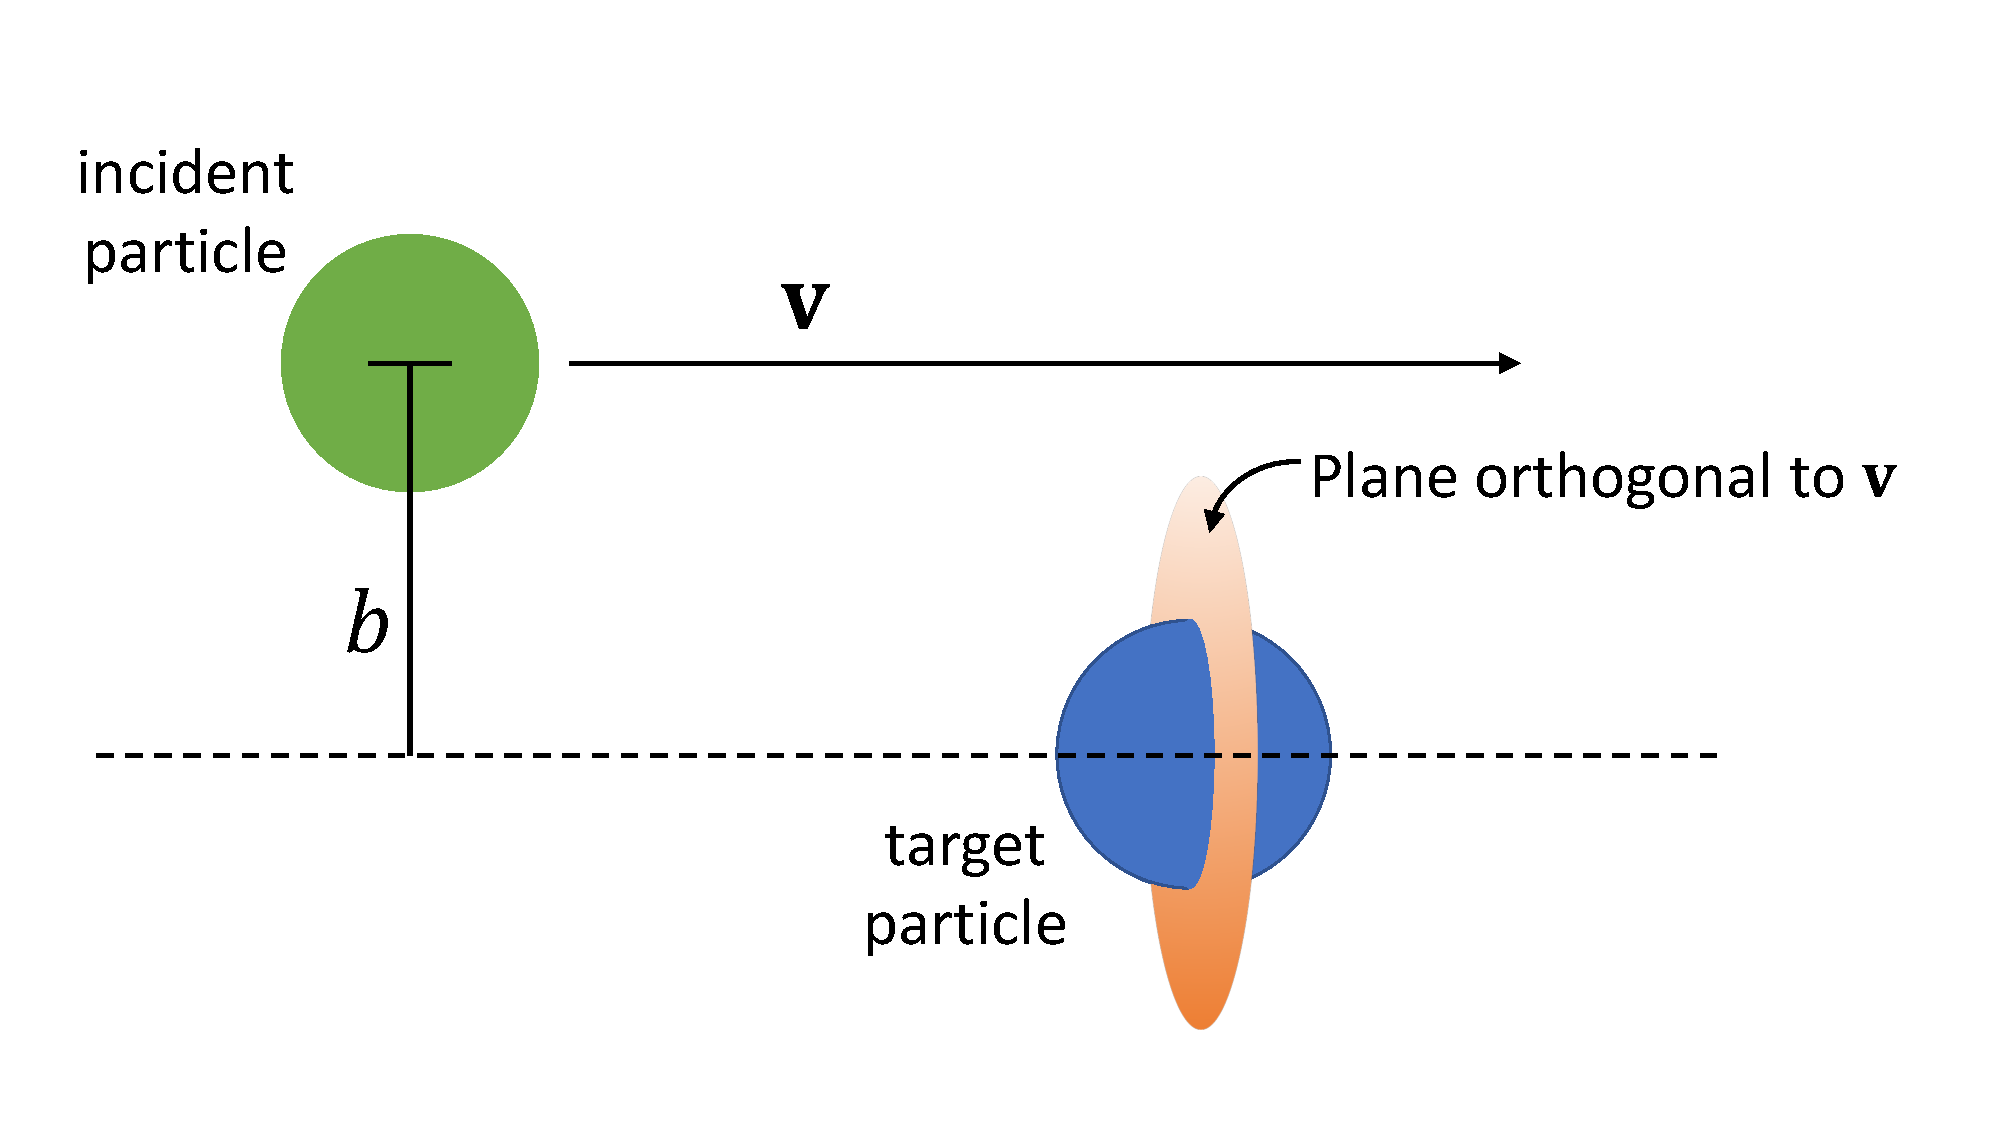
\includegraphics[width=10cm]{../../images/cross_section.pdf}
\caption{Cross section for particle interactions.}
\label{fig:cross_section}
\end{figure}

To quantify the above, the reader is referred to \cref{fig:cross_section}. Imagine an incident particle traveling towards a stationary target particle with an impact parameter $b$ and velocity $\vvec$ (if the target particle is not stationary, then $\vvec = \vvec_2 - \vvec_1$, where $\vvec_1$ is the velocity of the target particle and $\vvec_2$ is the velocity of the incident particle.) As shown in \cref{fig:cross_section}, the impact parameter is the perpendicular offset between the path of the incident particle, and the line parallel to the incident particle velocity that crosses the origin of the target particle (or the origin of the force field of the target particle). To determine the cross section, we ask the following question: for a particle with impact parameter $b$ and velocity magnitude $v = |\vvec|$, does it interact with the target particle? Let's say it does not interact, then the infinitesimal surface located at $b$, i.e.\@ $b db d\phi$ for cylindrical coordinates, does not contribute to the cross section. If it does interact, then $b db d\phi$ does contribute to the cross section. To obtain the total cross section $\sigma = \sigma(v)$, we sum over all infinitesimal areas $b db d\phi$, but account whether a particle at a given $b$ interacts or not with the target particle. This is expressed mathematically as
\begin{equation}
\label{eq:def_cross_section}
    \sigma = \int_0^{2\pi} \int_0^\infty F(v,b) \, b db d\phi.
\end{equation}
In the above $F(v,b) = 1$ if an incident particle with impact parameter $b$ and velocity $v$ interacts with the target particle, and $F(v,b) = 0$ if it does not. However, in reality, $F(v,b)$ is not necessarily binary, and can take other values besides 0 and 1.

An example of $F(v,b)$ is that corresponding to particles that are hard spheres with radius R. For this case, $F(v,b) = H(2R - b)$, where $H$ is the heaviside function. Thus,
\begin{equation}
    \sigma = \int_0^{2\pi} \int_0^\infty H(2R-b) \, b db d\phi = 2\pi \int_0^{2R} b db = \pi (2R)^2,
\end{equation}
as expected.

%-------------------------------------------------------------------------------
\section{Mean free path, collision time, and collision frequency}
%-------------------------------------------------------------------------------
The cross section then defines the mean free path $\lambda_m$, collision time $\tau_m$ and collision frequency $\nu_m$. These are given by
\begin{equation}
    \lambda_m = \frac{1}{n_1 \sigma},
\end{equation}
\begin{equation}
    \tau_m = \frac{\lambda_m}{v} = \frac{1}{n_1 \sigma v},
\end{equation}
and
\begin{equation}
    \nu_{m} = \frac{1}{\tau_m} = n_1 \sigma v.
\end{equation}

%--------------------------------------------------------------------------
\section{Coulomb scattering}
%--------------------------------------------------------------------------
%--------------------------------------------
\subsection{Particle equations}
%--------------------------------------------
Consider two particles, with positions $\rvec_1=\rvec_1(t)$ and $\rvec_2=\rvec_2(t)$, velocities $\vvec_1=\vvec_1(t)$ and $\vvec_2=\vvec_2(t)$, charges $q_1$ and $q_2$, and masses $m_1$ and $m_2$, respectively. Their positions and velocities are governed by the following equations 
\begin{equation}
    \label{eq:particle_1_pos}
    \frac{d \rvec_1}{dt} = \vvec_1,
\end{equation}
\begin{equation}
    \label{eq:particle_2_pos}
    \frac{d \rvec_2}{dt} = \vvec_2,
\end{equation}
\begin{equation}
    \label{eq:particle_1_vel}
    m_1 \frac{d\vvec_1}{dt} = -\frac{q_1 q_2}{4 \pi \epsilon} \frac{\rvec_2 - \rvec_1}{\left | \rvec_2 - \rvec_1 \right |^3},
\end{equation}
\begin{equation}
    \label{eq:particle_2_vel}
    m_2 \frac{d\vvec_2}{dt} = -\frac{q_1 q_2}{4 \pi \epsilon} \frac{\rvec_1 - \rvec_2}{\left | \rvec_1 - \rvec_2 \right |^3}.
\end{equation}
We note that the above system consists of twelve equations for twelve unknowns. We now introduce the center-of-mass position $\Rvec = \Rvec(t)$, the center-of-mass velocity $\Vvec = \Vvec(t)$, the shifted position $\rvec = \rvec(t)$ and the shifted velocity $\vvec = \vvec(t)$ as follows
\begin{equation}
    \Rvec = \frac{m_1 \rvec_1 + m_2 \rvec_2}{m_1 + m_2} \qquad \rvec = \rvec_1 - \rvec_2,
\end{equation}
\begin{equation}
    \Vvec = \frac{m_1 \vvec_1 + m_2 \vvec_2}{m_1 + m_2} \qquad \vvec = \vvec_1 - \vvec_2
\end{equation}
Thus, in terms of these new four variables, the particle equations can be written as
\begin{equation}
    \frac{d \Rvec}{dt} = \Vvec,
\end{equation}
\begin{equation}
    \frac{d \Vvec}{dt} = 0 ,
\end{equation}
\begin{equation}
    \label{eq:particle_pos}
    \frac{d \rvec}{dt} = \vvec,
\end{equation}
\begin{equation}
    \label{eq:particle_vel}
    \frac{d \vvec}{dt} = \frac{q_1 q_2}{4\pi \epsilon_0 m_r} \frac{\rvec}{r^3},
\end{equation}
where the reduced mass $m_r$ is given by
\begin{equation}
    \frac{1}{m_r} = \frac{1}{m_1} + \frac{1}{m_2}.
\end{equation}
The first two equations above give the trivial solution $\Vvec = $ constant and $\Rvec$ = $\Rvec(0) + \Vvec t$. Thus, we have reduced the problem from twelve unknowns to six unknowns, namely $\rvec$ and $\vvec$.

%--------------------------------------------
\subsection{Conservation of energy}
%--------------------------------------------
Dotting \cref{eq:particle_vel} by $\vvec$ gives 
\begin{align}
    \vvec \cdot \frac{d \vvec}{dt} &= \frac{q_1 q_2}{4 \pi \epsilon_0 m_r} \vvec \cdot \frac{\rvec}{r^3} \nonumber \\
    &= \frac{q_1 q_2}{4 \pi \epsilon_0 m_r} \frac{d\rvec}{dt} \cdot \frac{\rvec}{r^3} \nonumber \\
    &= \frac{q_1 q_2}{4 \pi \epsilon_0 m_r} \frac{1}{2} \frac{dr^2}{dt} \frac{1}{r^3} \nonumber \\
    &= \frac{q_1 q_2}{4 \pi \epsilon_0 m_r} \frac{1}{r^2} \frac{dr}{dt} \nonumber \\
    &= -\frac{q_1 q_2}{4 \pi \epsilon_0 m_r} \frac{d}{dt} \left ( \frac{1}{r} \right ).
\end{align} 
For the left hand side above we have
\begin{equation}
    \vvec \cdot \frac{d \vvec}{dt} = \frac{1}{2} \frac{d v^2}{dt},
\end{equation}
and thus we obtain the following expression for conservation of energy
\begin{equation}
    \frac{d}{dt} \left ( \frac{1}{2} m_r v^2 + \frac{q_1 q_2}{4 \pi \epsilon_0} \frac{1}{r} \right ) = 0.
\end{equation}

%--------------------------------------------
\subsection{Conservation of momentum}
%--------------------------------------------
Crossing \cref{eq:particle_vel} by $\rvec$ gives
\begin{equation}
    \rvec \times \frac{d \vvec}{dt} = \frac{q_1 q_2}{4 \pi \epsilon_0 m_r} \frac{\rvec \times \rvec}{r^3} = 0,
\end{equation}
and thus
\begin{equation}
    \frac{d}{dt} \left [ m_r \left ( \rvec \times \vvec \right ) \right ] = 0.
\end{equation}
That is, angular momentum is conserved. A consequence of this is that the vector $\rvec \times \vvec$ is always pointing in the same direction. Thus, if $\rvec(0)$ and $\vvec(0)$ form a plane, then $\rvec(t)$ and $\vvec(t)$ need to reside within that same plane for all times $t$ so that $\rvec(t) \times \vvec(t)$ points in the same direction as $\rvec(0) \times \vvec(0)$. Therefore, the evolution of the position and velocity are confined to a plane and the problem can be reduced from six unknowns to four unknowns. This planar encounter is depicted in \cref{fig:coulomb_scattering}.
\begin{figure}[ht]
    \centering
    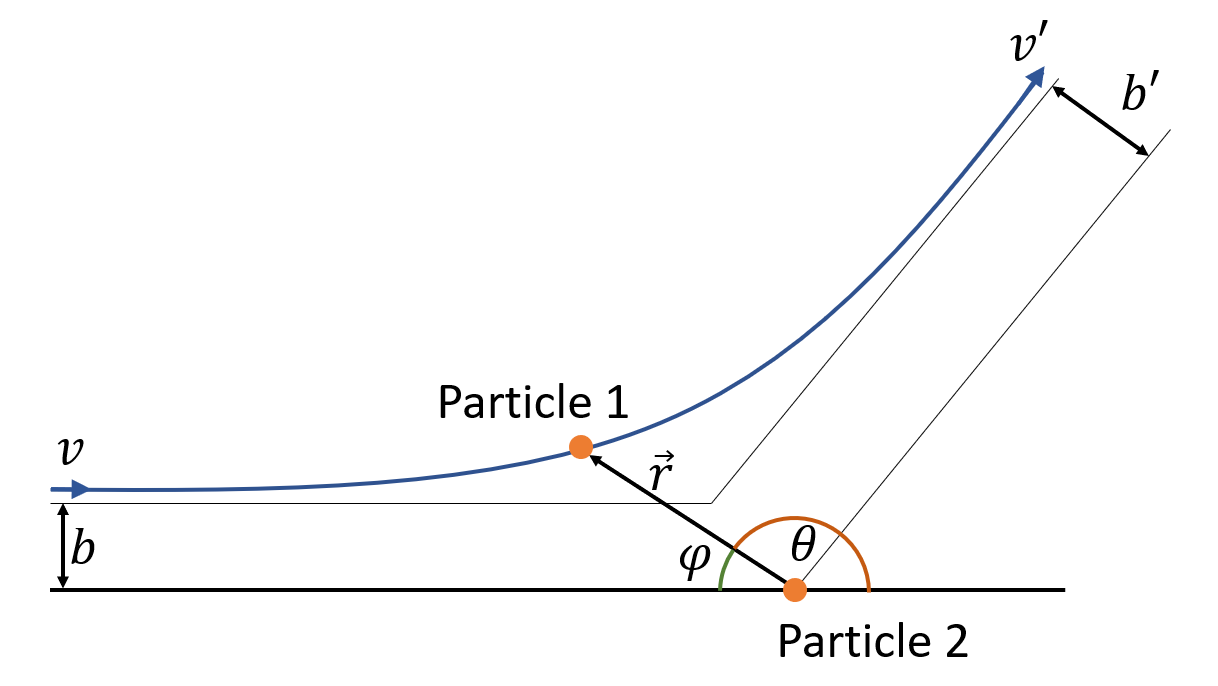
\includegraphics[width=10cm]{../../images/coulomb_scattering.png}
    \caption{Depiction of Coulomb scattering.}
    \label{fig:coulomb_scattering}
    \end{figure}

%--------------------------------------------
\subsection{Polar coordinates}
%--------------------------------------------
\begin{figure}[ht]
    \centering
    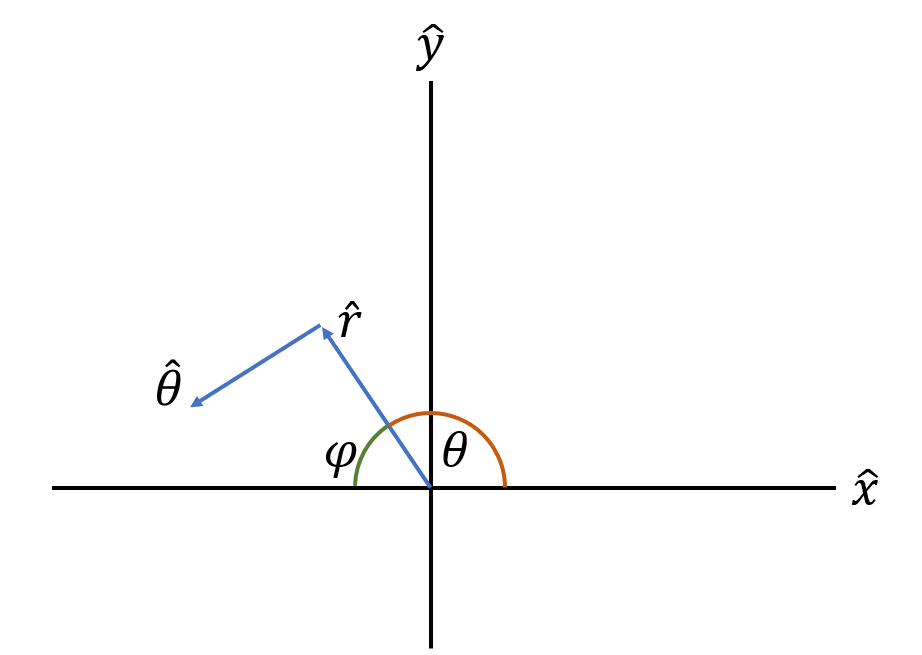
\includegraphics[width=10cm]{../../images/polar_coordinates.png}
    \caption{Polar coordinates in plane of interaction.}
    \label{fig:polar_coordinates}
    \end{figure}

We re-orient the plane of interaction (referred to above) so that it is orthogonal to the $\hat{\zvec}$ direction. Using polar coordinates, as shown in \cref{fig:polar_coordinates}, we get
\begin{equation}
    r_x = r \cos \theta = r \cos ( \pi - \varphi ) = -r \cos \varphi,
\end{equation}
\begin{equation}
    r_y = r \sin \theta = r \sin ( \pi - \varphi ) = r \sin \varphi.
\end{equation}

Also, since $\rvec = r \hat{\rvec}$, we have
\begin{align}
    \vvec = &\frac{d \rvec}{dt} = \frac{dr}{dt} \hat{\rvec} + r \frac{d\hat{\rvec}}{dt} \nonumber \\
    &= \frac{d r}{dt} \hat{\rvec} + r \frac{d\hat{\rvec}}{d\theta} \frac{d\theta}{dt} \nonumber \\
    &= \frac{dr}{dt} \hat{\rvec} + r \frac{d \theta}{dt} \hat{\bm{\theta}},
\end{align}
and
\begin{align}
    \frac{d \vvec}{dt} &= \frac{d^2r}{dt^2} \hat{\rvec} + \frac{dr}{dt} \frac{d\hat{\rvec}}{dt} + \frac{d}{dt} \left ( r \frac{d\theta}{dt} \right ) \hat{\bm{\theta}} + r \frac{d \theta}{dt} \frac{d \hat{\bm{\theta}}}{dt} \nonumber \\
    &= \frac{d^2 r}{dt^2} \hat{\rvec} + \frac{dr}{dt} \frac{d\hat{\rvec}}{d\theta} \frac{d\theta}{dt} + \frac{d}{dt} \left ( r \frac{d\theta}{dt} \right ) \hat{\bm{\theta}} + r \frac{d \theta}{dt} \frac{d \hat{\bm{\theta}}}{d\theta} \frac{d \theta}{dt} \nonumber \\
    &= \frac{d^2r}{dt^2} \hat{\rvec} + \frac{dr}{dt} \frac{d\theta}{dt} \hat{\bm{\theta}} + \frac{d}{dt} \left ( r \frac{d\theta}{dt} \right ) \hat{\bm{\theta}} - r \left ( \frac{d\theta}{dt} \right ) ^2 \hat{\rvec}.
\end{align}

%--------------------------------------------
\subsection{The force equation}
%--------------------------------------------
The radial component of \cref{eq:particle_vel} thus becomes 
\begin{equation}
    \frac{d^2 r}{dt^2} - r \left ( \frac{d\theta}{dt} \right )^2 = \frac{q_1 q_2}{4 \pi \epsilon_0 m_r} \frac{1}{r^2}.
\end{equation}
Since $\theta = \pi - \varphi$, we have
\begin{equation}
    \label{eq:particle_position_ode}
    \frac{d^2 r}{dt^2} - r \left ( \frac{d\varphi}{dt} \right )^2 = \frac{q_1 q_2}{4 \pi \epsilon_0 m_r} \frac{1}{r^2}.
\end{equation}

%--------------------------------------------
\subsection{The angular momentum equation}
%--------------------------------------------
Using polar coordinates, we obtain
\begin{equation}
    m_r \rvec \times \vvec = m_r r \hat{\rvec} \times \left ( \frac{dr}{dt} \hat{\rvec} + r \frac{d\theta}{dt} \hat{\bm{\theta}} \right ) = m_r r^2 \frac{d\theta}{dt} \hat{\zvec}
\end{equation}
Since angular momentum $m_r \rvec \times \vvec$ is conserved, we have
\begin{equation}
    \label{eq:particle_cons_angular_polar}
    m_r r^2 \frac{d\varphi}{dt} = L = constant.
\end{equation}
We note here that $L$ is positive since $d\varphi/dt$ is positive. Also, we have 
\begin{equation}
    \label{eq:particle_angular_sign}
    m_r \rvec \times \vvec = -L \hat{\zvec},
\end{equation}
that is, the angular momentum is in the negative $\hat{\zvec}$ direction.

%--------------------------------------------
\subsection{Particle trajectory}
%--------------------------------------------
The goal is to find the radial position of the particle as a function of its angular orientation. That is, we want to find $\tilde{r} = \tilde{r}(\tilde{\varphi})$ such that
\begin{equation}
    \label{eq:particle_position_angle}
    r(t) = \tilde{r}(\varphi(t)).
\end{equation}
To simplify the math, we introduce $\tilde{u} = \tilde{u}(\tilde{\varphi})$ such that $\tilde{u} = 1 / \tilde{r}$. Thus
\begin{equation}
    \frac{d \tilde{u}}{d\tilde{\varphi}} = -\frac{1}{\tilde{r}^2} \frac{d \tilde{r}}{d\tilde{\varphi}},
\end{equation}
or, after re-arranging
\begin{equation}
    \label{eq:rgrad_vs_ugrad}
    \frac{d \tilde{r}}{d\tilde{\varphi}} = -\frac{1}{\tilde{u}^2} \frac{d \tilde{u}}{d\tilde{\varphi}}.
\end{equation}

We now proceed as follows. Taking the derivative of $r$, we get
\begin{align}
    \label{eq:particle_derivation_1}
    \frac{dr}{dt} &= \left ( \frac{d \tilde{r}}{d\tilde{\varphi}} \right )_{\tilde{\varphi} = \varphi(t)} \frac{d \varphi}{dt} &&[\cref{eq:particle_position_angle}] \nonumber \\
    &= \left ( -\frac{1}{\tilde{u}^2} \frac{d\tilde{u}}{d\tilde{\varphi}} \right )_{\tilde{\varphi} = \varphi(t)} \frac{d \varphi}{dt} &&[\cref{eq:rgrad_vs_ugrad}]\nonumber \\ 
    &= \left ( -\frac{1}{\tilde{u}^2} \frac{d\tilde{u}}{d\tilde{\varphi}} \right )_{\tilde{\varphi} = \varphi(t)} \frac{L}{m_r r^2} &&[\cref{eq:particle_cons_angular_polar}] \nonumber \\
    &= \left ( -\frac{1}{\tilde{u}^2} \frac{d\tilde{u}}{d\tilde{\varphi}} \frac{L}{m_r \tilde{r}^2} \right )_{\tilde{\varphi} = \varphi(t)} &&[\cref{eq:particle_position_angle}] \nonumber \\
    &= \left ( - \frac{d\tilde{u}}{d\tilde{\varphi}} \frac{L}{m_r} \right )_{\tilde{\varphi} = \varphi(t)}
\end{align}
Taking the derivative of the above, we get
\begin{align}
    \frac{d}{dt} \frac{dr}{dt} &= \left [ \frac{d}{d\tilde{\varphi}} \left ( - \frac{d\tilde{u}}{d\tilde{\varphi}} \frac{L}{m_r} \right ) \right ]_{\tilde{\varphi} = \varphi(t)} \frac{d \varphi}{dt} \nonumber \\
    &= \left ( - \frac{d^2 \tilde{u}}{d\tilde{\varphi}^2} \frac{L}{m_r} \right )_{\tilde{\varphi} = \varphi(t)} \frac{L}{m_r r^2} && [\cref{eq:particle_cons_angular_polar}] \nonumber \\
    &= \left ( - \frac{d^2 \tilde{u}}{d\tilde{\varphi}^2} \frac{L}{m_r} \frac{L}{m_r \tilde{r}^2} \right )_{\tilde{\varphi} = \varphi(t)} && [\cref{eq:particle_position_angle}] \nonumber \\
    &= \left ( - \frac{d^2 \tilde{u}}{d\tilde{\varphi}^2} \frac{L^2 \tilde{u}^2}{m_r^2} \right )_{\tilde{\varphi} = \varphi(t)}
\end{align}
Plugging the last relation into \cref{eq:particle_position_ode} gives
\begin{equation}
    \left [ - \frac{d^2 \tilde{u}}{d\tilde{\varphi}^2} \frac{L^2 \tilde{u}^2}{m_r^2} - \frac{1}{\tilde{u}} \left ( \frac{L \tilde{u}^2}{m_r} \right )^2 \right ]_{\tilde{\varphi} = \varphi(t)} = \left ( \frac{q_1 q_2}{4 \pi \epsilon_0 m_r} \tilde{u}^2 \right )_{\tilde{\varphi} = \varphi(t)},
\end{equation}
which, upon re-arranging and dropping the $\varphi(t)$ dependance, becomes
\begin{equation}
    \frac{d^2 \tilde{u}}{d \tilde{\varphi}^2} + \tilde{u} = -\frac{q_1 q_2 m_r}{4 \pi \epsilon_0 L^2}
\end{equation}

Using \cref{eq:particle_angular_sign}, we have
\begin{align}
    \label{eq:particle_momentum_impact}
    L &= -m_r ( \rvec \times \vvec )\cdot \hat{\zvec} \nonumber \\
    &= -m_r [\sin(-\theta) r v_0 \hat{\zvec} ] \cdot \hat{\zvec} \nonumber \\
    &= m_r\sin(\theta) r v_0 \nonumber \\
    &= m_r\sin(\pi - \varphi) r v_0 \nonumber \\
    &= m_r\sin\varphi r v_0 \nonumber \\
    &= m_r b v_0.
\end{align}
Thus, we write the evolution equation for $\tilde{u}$ as
\begin{equation}
    \frac{d^2 \tilde{u}}{d \tilde{\varphi}^2} + \tilde{u} = -\frac{q_1 q_2}{4 \pi \epsilon_0 m_r b^2 v_0^2}.
\end{equation}
Introducing the notation
\begin{equation}
    b_{90} = \frac{q_1 q_2}{4 \pi \epsilon_0 m_r v_0^2},
\end{equation}
the evolution equation for $\tilde{u}$ can be simply expressed as
\begin{equation}
    \label{eq:particle_u_equation}
    \frac{d^2 \tilde{u}}{d \tilde{\varphi}^2} + \tilde{u} = -\frac{b_{90}}{b^2}.
\end{equation}

The boundary conditions for \cref{eq:particle_u_equation} are as follows
\begin{equation}
    \label{eq:particle_bc_1}
    \text{as } \varphi(t) \to 0, \quad r(t) \to \infty
\end{equation}
\begin{equation}
    \label{eq:particle_bc_2}
    \text{as } \varphi(t) \to 0, \quad \frac{dr(t)}{dt} \to -v_0
\end{equation}
Given \cref{eq:particle_position_angle}, \cref{eq:particle_bc_1} can only be satisfied if as $\tilde{\varphi} \to 0$, $\tilde{r} \to \infty$. Thus, we also have, as $\tilde{\varphi} \to 0$, $\tilde{u} \to 0$. Similarly, given \cref{eq:particle_derivation_1}, \cref{eq:particle_bc_2} can only be satisfied if as $\tilde{\varphi} \to 0$
\begin{equation}
    \frac{d\tilde{u}}{d\tilde{\varphi}} \frac{L}{m_r} \to v_0.
\end{equation}
Using \cref{eq:particle_momentum_impact} we rewrite the above as 
\begin{equation}
    \frac{d\tilde{u}}{d\tilde{\varphi}} \to \frac{1}{b}.
\end{equation}

The general solution to \cref{eq:particle_u_equation} is 
\begin{equation}
    \tilde{u} = A \cos \tilde{\varphi} + B \sin \tilde{\varphi} - \frac{b_{90}}{b^2}.
\end{equation}
Applying the boundary conditions, we get
\begin{equation}
    \tilde{u} = \frac{b_{90}}{b^2} \cos \tilde{\varphi} + \frac{1}{b} \sin \tilde{\varphi} - \frac{b_{90}}{b^2},
\end{equation}
which we finally re-write as
\begin{equation}
    \frac{1}{\tilde{r}} = \frac{1}{b} \sin \tilde{\varphi} + \frac{b_{90}}{b^2} \left ( \cos \tilde{\varphi} - 1 \right ).
\end{equation}

%-------------------------------------------------------------------------------
\section{Collision integral}
%-------------------------------------------------------------------------------
\begin{equation}
    \Omega_{\alpha \beta}^{(lk)} = \sqrt{ \frac{k_B T}{2 \pi M_{\alpha \beta}} } \int_0^\infty e^{-g^2} g^{2k+3} \phi_{\alpha \beta}^{(l)} \, dg.
\end{equation}
In the above $M_{\alpha \beta}$ is the reduced mass, given by
\begin{equation}
    M_{\alpha \beta} = \frac{M_\alpha M_\beta}{M_\alpha + M_\beta},
\end{equation}
and $\phi^{(l)}_{\alpha \beta}$ is the collision cross section for a given velocity, and is computed as
\begin{equation}
    \phi_{\alpha \beta}^{(l)} = 2 \pi \int_0^\infty \left ( 1 - \cos^l \chi_{\alpha \beta} \right ) b \, db.
\end{equation}
The scattering angle $\chi_{\alpha \beta}$ is given by
\begin{equation}
    \chi_{\alpha \beta} = \pi - 2 \int_{r_{\alpha \beta}^{\text{min}}}^\infty \frac{b}{r^2 \left [ 1 - \frac{b^2}{r^2} - \frac{V_{\alpha \beta (r)}}{g^2 k_B T} \right ]^{1/2} } \, dr.
\end{equation}

For a Coulombic interaction between ions, we can define the natural scale fore the cross-sectional area as
\begin{equation}
    \phi^{(0)}_{\alpha \beta} = \frac{ \pi \left (Z_\alpha Z_\beta e^2 \right)^2}{ \left(2 k_B T\right)^2}.
\end{equation}
Given this definition, we express the collision integral as
\begin{equation}
    \Omega_{\alpha \beta} = \sqrt{ \frac{\pi }{M_{\alpha \beta}}} \frac{( Z_\alpha Z_\beta e^2)^2 }{(2 k_B T )^{3/2}} \mathcal{F}^{lk}_{\alpha \beta},
\end{equation}
where
\begin{equation}
    \mathcal{F}^{(lk)}_{\alpha \beta} = \frac{1}{2 \phi_0} \int_0^\infty e^{-g^2} g^{2k+3} \phi_{\alpha \beta}^{(l)} \, dg
\end{equation}
We note that $\mathcal{F}^{(lk)}_{\alpha \beta} = 4 \mathcal{K}_{lk}(g_{\alpha \beta})$, where $\mathcal{K}_{lk}(g_{\alpha \beta})$ is the notation from the Stanton-Murillo paper.

%----------------------------------------------------------------------------------------------------------------------
\chapter{Transport coefficients}
%----------------------------------------------------------------------------------------------------------------------

%----------------------------------------------------------------------------------------------------------------------
\chapter{Coupling coefficients}
%----------------------------------------------------------------------------------------------------------------------
%-------------------------------------------------------------------------------
\section{Momentum exchange collision frequency $\nu_{ei}$}
%-------------------------------------------------------------------------------
%-------------------------------------------------------------------------------
\section{Electron-ion thermal coupling $w_{ei}$}
%-------------------------------------------------------------------------------

%----------------------------------------------------------------------------------------------------------------------
\chapter{Ionization}
%----------------------------------------------------------------------------------------------------------------------

%----------------------------------------------------------------------------------------------------------------------
\chapter{Warm dense matter}
%----------------------------------------------------------------------------------------------------------------------
%-------------------------------------------------------------------------------
\section{Coupling parameter}
%-------------------------------------------------------------------------------
%--------------------------------------------
\subsection{Definition}
%--------------------------------------------
We can define two types of Coulomb interactions: strong and weak. Strong Coulomb interactions are those for which the particle's Coulomb potential energy is larger than its kinetic energy, and viceversa for weak Coulomb interactions. Thus, we can also define two types of plasma regimes:
\begin{itemize}
    \item Strongly-coupled plasmas: plasmas where the Coulomb interactions are mostly strong and thus drive the dynamics of its evolution. Coulomb interactions tend to be strong when the inter-particle distances are small, and thus this regime would be dominated by \textit{short-range} interactions. These plasmas are also described as exhibiting \textit{collisional} behavior, since a strong Coulomb interaction essentially means a collision has occurred.
    \item Weakly-coupled plasmas: plasmas where the Coulomb interactions are mostly weak, and as a result do not drive the dynamics of its evolution. The plasma dynamics are instead driven by \textit{long-range} effects caused by smooth electromagnetic fields that result from integrating a large number of particles. These plasmas are also described as exhibiting \textit{collective} behavior, since the long-range electromagnetic fields follow from the collective integration of many particles.
\end{itemize}

We describe an approximate Coulomb potential energy for particles in a plasma as
\begin{equation}
    \text{U} =  \frac{q_\alpha^2}{4 \pi \epsilon_0 a_\alpha}.
\end{equation}
The impact parameter that has been used above is $a_\alpha$, the sphere radius. This provides a decent measure on the average spacing between particles in a plasma. Since the volume of a single particle is $1/n_\alpha$, and if we assume that this volume is given by $4/3 \pi a_\alpha^3$, then equating these two gives the expression for the sphere radius
\begin{equation}
    a_\alpha = \left ( \frac{3}{4 \pi n_\alpha} \right )^{1/3}.
\end{equation}
The thermal velocity of a particle is given by
\begin{equation}
    v_{T_\alpha} = \sqrt{\frac{k_B T_\alpha}{m_\alpha}}
\end{equation}
A measure of the kinetic energy of a particle is given in terms of the thermal velocity as shown below
\begin{equation}
    \text{K} = m_\alpha v_{T_\alpha}^2 = k_B T_\alpha
\end{equation}
The ratio of the particle's Coulomb potential energy and its kinetic energy is referred to as the coupling parameter $\Gamma_\alpha$. That is 
\begin{equation}
    \Gamma_\alpha = \frac{q_\alpha^2}{4 \pi \epsilon_0 a_\alpha k_B T_\alpha}.
\end{equation}
$\Gamma_\alpha > 1$ denotes a strongly coupled plasma, and $\Gamma_\alpha < 1$ denotes a weakly coupled plasma. 

%--------------------------------------------
\subsection{The plasma parameter}
%--------------------------------------------
There is a one to one relationship between the coupling parameter and the standard plasma parameter. We begin with the electron plasma frequency, which is defined as follows
\begin{equation}
    w_{p\alpha} = \sqrt{\dfrac{n_\alpha q_\alpha^2}{m_\alpha \epsilon_0}}.
\end{equation}

With the above two scales, we can define the Debye length as
\begin{equation}
    \lambda_{D\alpha} = \frac{v_{T\alpha}}{w_{p\alpha}} = \sqrt{ \dfrac{\epsilon_0 k_B T_\alpha}{ n_\alpha q_\alpha^2}}.
\end{equation}
We note that the total Debye length would be
\begin{equation}
    \frac{1}{\lambda_D^2} = \sum_\alpha \frac{1}{\lambda_{D\alpha}^2}.
\end{equation}
Using the Debye length, one can define the plasma parameter as
\begin{equation}
    \Lambda_\alpha = \frac{4}{3} \pi \lambda_{D\alpha}^3 n_\alpha
\end{equation}
Simple algebra then shows that $\Gamma_\alpha = (1/3) \Lambda_\alpha^{-2/3}$. Thus, the coupling and plasma parameters are inversely proportional to each other. $\Lambda_\alpha < 1$ implies strongly-coupled plasmas, and $\Lambda_\alpha > 1$ weakly-coupled plasmas. Since $\Lambda_\alpha$ represents the number of particles per Debye sphere, it is interesting to see that a large number of particles within such a sphere is needed to be in the weakly-coupled-plasma regime. However, this does not correspond to a plasma with large density, in fact, it corresponds to the opposite. The explicit $n_\alpha$ term in the definition $\Lambda_\alpha = (4/3) \pi \lambda^3_{D\alpha} n_\alpha$ is dominated by the $n_\alpha$ in the denominator of $\lambda_{D\alpha}$. In other words, low plasma densities lead to large Debye spheres, which in turn leads to many particles per Debye sphere, and hence a weakly-coupled plasma.

%-------------------------------------------------------------------------------
\section{Electron degeneracy}
%-------------------------------------------------------------------------------
\begin{itemize}
    \item DeBroglie wavelength
    \begin{equation}
        \lambda_{B\alpha} = \dfrac{h}{\sqrt{2 \pi} m_\alpha v_{T\alpha}}
    \end{equation}
    \item Quantum plasma parameter
    \begin{equation}
        \chi_\alpha = \frac{4}{3} \pi \lambda_{B\alpha}^3 n_\alpha
    \end{equation}
    
    \item Fermi energy for electrons:
    \begin{equation}
        E_{fe} = \frac{\hbar^2}{2m_e} \left ( 3 \pi^2 n_e \right)^{2/3}
    \end{equation}

    \item Degeneracy parameter for electrons:
    \begin{equation}
        \Theta_e = \frac{k_B T_e}{E_{fe}} = \left( \frac{2^{10} \pi}{3^4} \right)^{1/3} \chi_e^{-2/3}
    \end{equation}
\end{itemize}

\end{document}